\documentclass[tikz,border=10pt]{standalone}
\usepackage{tikz}
\usetikzlibrary{shapes,arrows,positioning,shadows}

\begin{document}

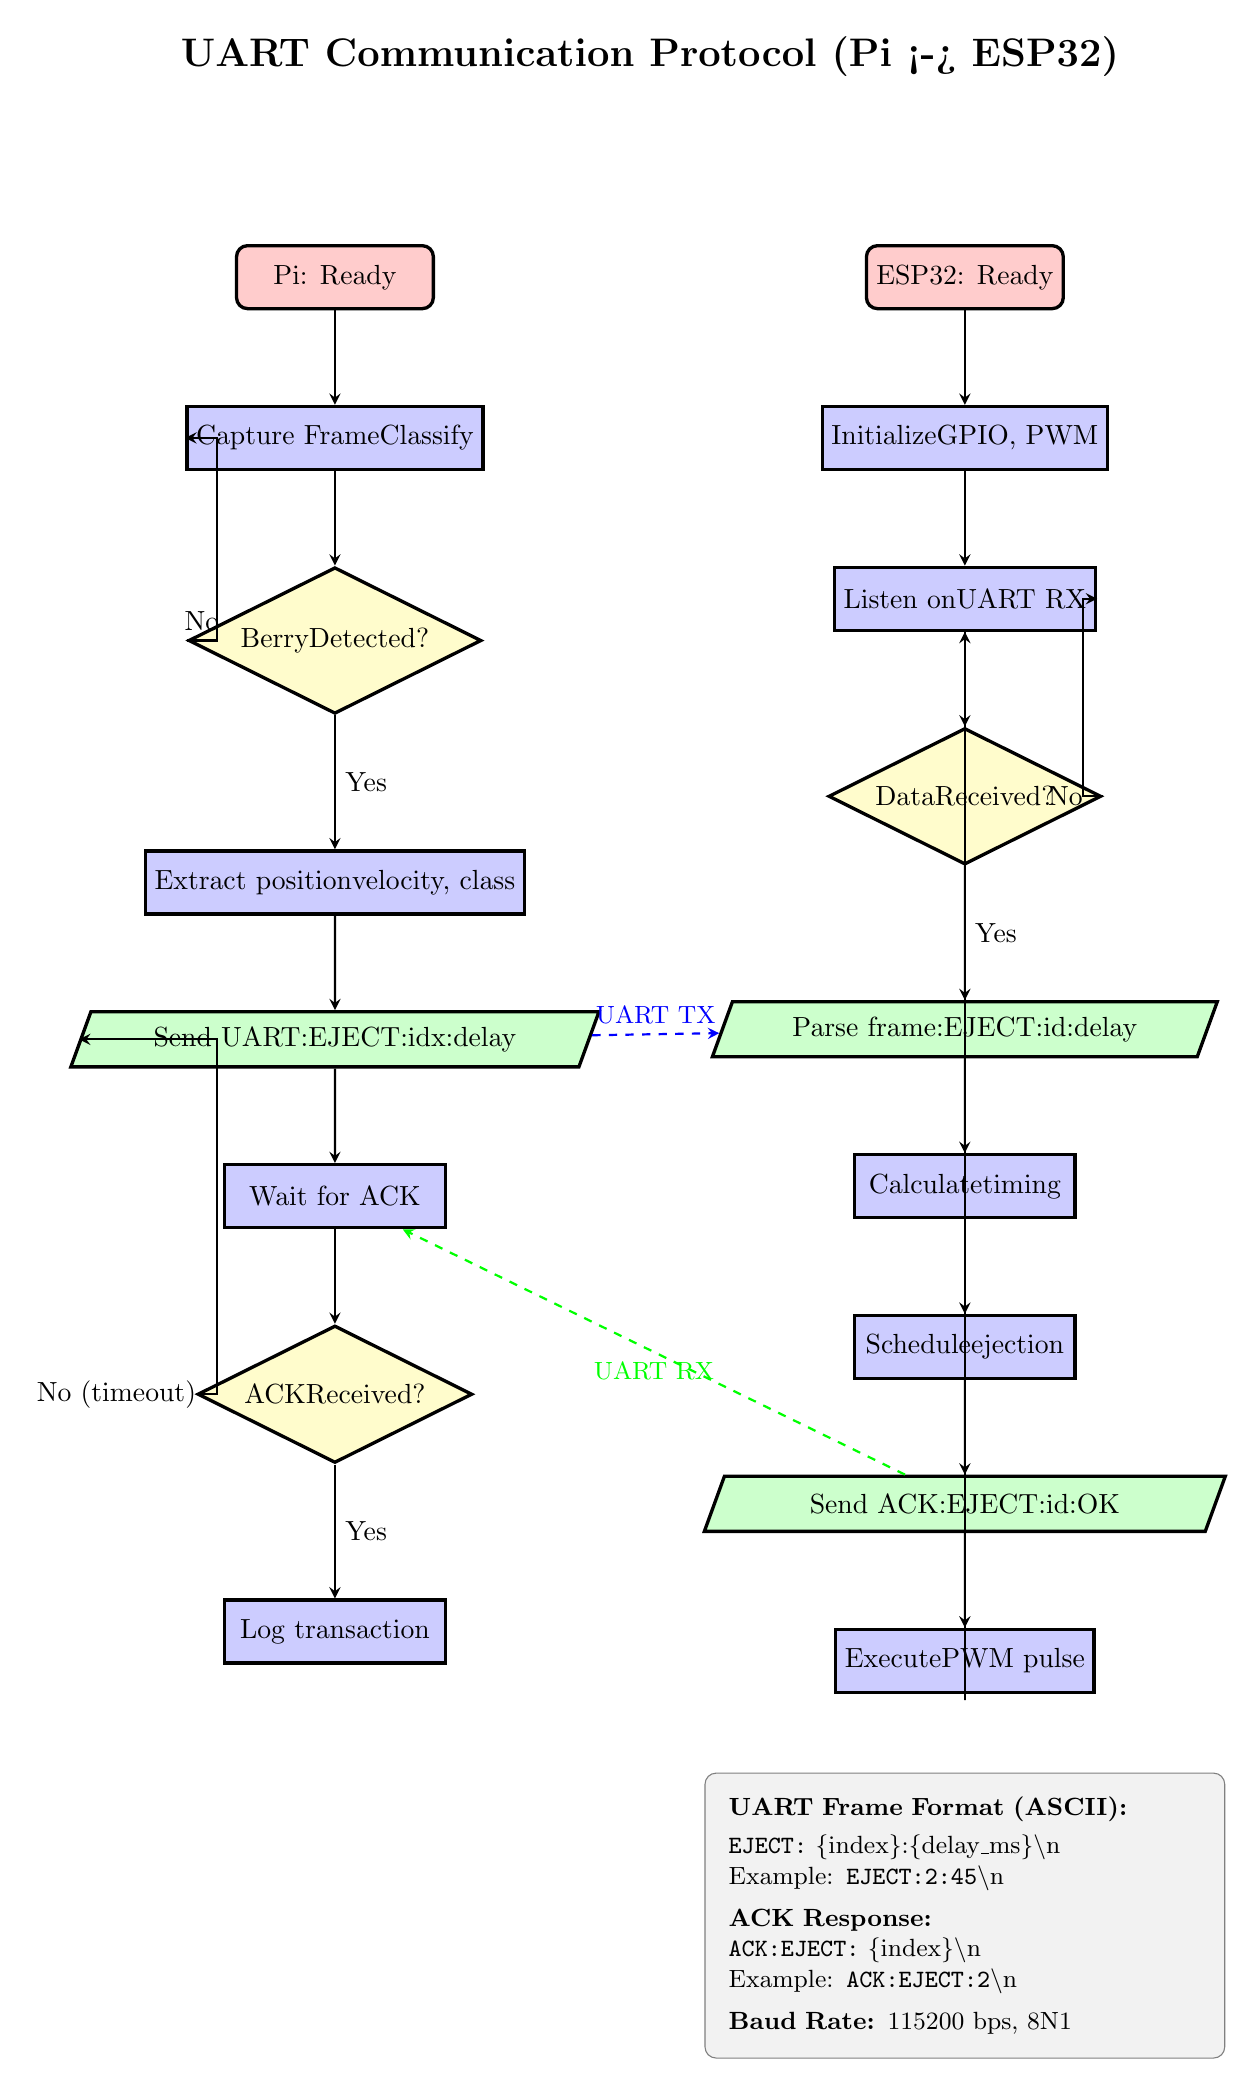
\begin{tikzpicture}[
    node distance=1.2cm,
    startstop/.style={rectangle, rounded corners, minimum width=2.5cm, minimum height=0.8cm, text centered, draw=black, fill=red!20, very thick},
    process/.style={rectangle, minimum width=2.8cm, minimum height=0.8cm, text centered, draw=black, fill=blue!20, very thick},
    decision/.style={diamond, minimum width=2.5cm, minimum height=1cm, text centered, draw=black, fill=yellow!20, very thick, aspect=2},
    io/.style={trapezium, trapezium left angle=70, trapezium right angle=110, minimum width=2.5cm, minimum height=0.7cm, text centered, draw=black, fill=green!20, very thick},
    arrow/.style={thick,->,>=stealth},
    title/.style={font=\bfseries\Large}
]

% Title
\node[title] (title) {UART Communication Protocol (Pi <-> ESP32)};

% Left column: Raspberry Pi
\node[startstop, below=2cm of title, xshift=-4cm] (pi_start) {Pi: Ready};
\node[process, below=of pi_start] (pi_capture) {Capture Frame\\Classify};
\node[decision, below=of pi_capture] (pi_detect) {Berry\\Detected?};
\node[process, below=of pi_detect, yshift=-0.5cm] (pi_parse) {Extract position\\velocity, class};
\node[io, below=of pi_parse] (pi_send) {Send UART:\\EJECT:idx:delay};
\node[process, below=of pi_send] (pi_wait) {Wait for ACK};
\node[decision, below=of pi_wait] (pi_timeout) {ACK\\Received?};
\node[process, below=of pi_timeout, yshift=-0.5cm] (pi_log) {Log transaction};

% Right column: ESP32
\node[startstop, below=2cm of title, xshift=4cm] (esp_start) {ESP32: Ready};
\node[process, below=of esp_start] (esp_init) {Initialize\\GPIO, PWM};
\node[process, below=of esp_init] (esp_listen) {Listen on\\UART RX};
\node[decision, below=of esp_listen] (esp_data) {Data\\Received?};
\node[io, below=of esp_data, yshift=-0.5cm] (esp_parse) {Parse frame:\\EJECT:id:delay};
\node[process, below=of esp_parse] (esp_calc) {Calculate\\timing};
\node[process, below=of esp_calc] (esp_sched) {Schedule\\ejection};
\node[io, below=of esp_sched] (esp_ack) {Send ACK:\\EJECT:id:OK};
\node[process, below=of esp_ack] (esp_execute) {Execute\\PWM pulse};

% Arrows Pi side
\draw[arrow] (pi_start) -- (pi_capture);
\draw[arrow] (pi_capture) -- (pi_detect);
\draw[arrow] (pi_detect) -- node[right] {Yes} (pi_parse);
\draw[arrow] (pi_detect) -- node[above] {No} ++(-1.5,0) |- (pi_capture);
\draw[arrow] (pi_parse) -- (pi_send);
\draw[arrow] (pi_send) -- (pi_wait);
\draw[arrow] (pi_wait) -- (pi_timeout);
\draw[arrow] (pi_timeout) -- node[right] {Yes} (pi_log);
\draw[arrow] (pi_timeout) -- node[left] {No (timeout)} ++(-1.5,0) |- (pi_send);

% Arrows ESP32 side
\draw[arrow] (esp_start) -- (esp_init);
\draw[arrow] (esp_init) -- (esp_listen);
\draw[arrow] (esp_listen) -- (esp_data);
\draw[arrow] (esp_data) -- node[right] {Yes} (esp_parse);
\draw[arrow] (esp_data) -- node[left] {No} ++(1.5,0) |- (esp_listen);
\draw[arrow] (esp_parse) -- (esp_calc);
\draw[arrow] (esp_calc) -- (esp_sched);
\draw[arrow] (esp_sched) -- (esp_ack);
\draw[arrow] (esp_ack) -- (esp_execute);
\draw[arrow] (esp_execute) -- ++(0,-0.5) -| (esp_listen);

% Communication arrows (UART)
\draw[arrow, thick, dashed, blue] (pi_send) -- node[above, font=\small] {UART TX} (esp_parse);
\draw[arrow, thick, dashed, green] (esp_ack) -- node[below, font=\small] {UART RX} (pi_wait);

% Frame format box
\node[below=1cm of esp_execute, text width=6cm, draw=black!50, fill=gray!10, rounded corners, inner sep=0.3cm, anchor=north, font=\small] (frame) {
    \textbf{UART Frame Format (ASCII):}\\[0.1cm]
    \texttt{EJECT:} \{index\}:\{delay\_ms\}\textbackslash n\\
    Example: \texttt{EJECT:2:45}\textbackslash n\\[0.15cm]
    \textbf{ACK Response:}\\
    \texttt{ACK:EJECT:} \{index\}\textbackslash n\\
    Example: \texttt{ACK:EJECT:2}\textbackslash n\\[0.15cm]
    \textbf{Baud Rate:} 115200 bps, 8N1
};

\end{tikzpicture}

\end{document}
